 \section{Methodology}\label{sec:methodology}
  \subsection{The Setup}
  \begin{figure}[!htbp]
  	\centering 
	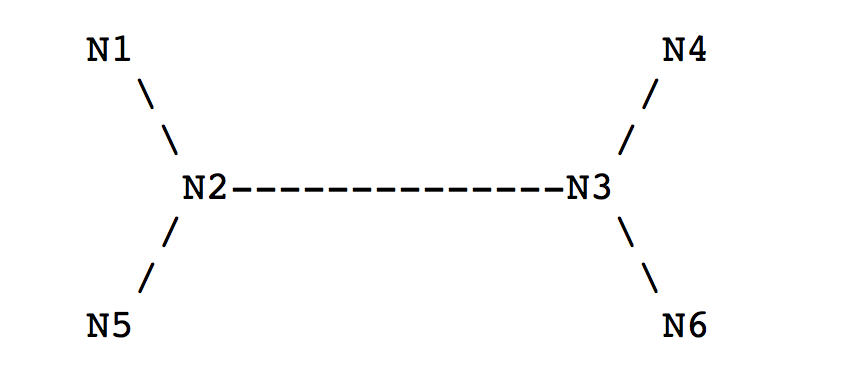
\includegraphics[scale=0.4]{setup.png}
	\caption{We attach TCP agent with FTP as the application, UDP with CBR to this topology.}
	\label{fig:setup}
\end{figure}
We use ns2 to create the topology in Figure \ref{fig:setup}. The setup consists of five different nodes, N1- N5. The link between each pair of nodes is a duplex link with a capacity of 10 Mb.
\subsection{Calculation}
NS2 trace files were used to calculate drop rate, average throughput, average latency and latency over time for different TCP variants and different queuing algorithms. 
\begin{enumerate}
\item \textbf{Average Throughput:}
\item \textbf{Latency:}
\item \textbf{Drop Rate:}
\end{enumerate}


 \subsection{TCP Performance Under Congestion}
This experiment was designed to test performance of different TCP variants Tahoe, Reno, NewReno and Vegas under various levels of congestions. TCP agents were attached to start at N1 and sink at N4. FTP application was attached to the TCP agent to simulate traffic that is typical of FTP. CBR flow was from N2 to N3 to create congestion in the link between N2 and N3. We varied the CBR rate from 1 Mbps to 10 Mbps to create various levels of congestion and simulated how each TCP variant performs by calculating the average throughput, average latency and the drop rate. We use a bash script to automate a series of experiments with varying TCP variant, CBR rate and CBR packet size. 
 \subsection{Fairness between TCP variants}
 \begin{enumerate}
\item Reno/Reno
\item NewReno/Reno
\item Vegas/Vegas
\item NewReno/Vegas
 \end{enumerate}
 \subsection{Influence of Queuing}
 
 For this experiment we set up 